\chapter{Conclusion}
\begin{flushright}
    \textit{''Well, I'm all for leaving \\
            and that being done,\\
            I've put in a request to take up my turn.''}\\
    Jethro Tull, A Passion Play, 1973
\end{flushright}



\section{Concluding Overview}
\subsection{Final Summary}
As the author of this manuscript easily recognized during proofreading, sifting through more than two hundred pages of early-career neuroscience is not exactly a straightforward ordeal. Although an attempt has been made to lower the attentional overhead involved in this reading by humoring the reader and by limiting the number of abbreviations, it is likely that days have elapsed between the beginning and the end of one's reading. As such, we would like to summarize, once last time, this manuscript

We first introduced the problem of inverse variance computations in vision by adopting a Marr-like approach in chapter 2. This introduced a study of the nature of natural images in chapter 3, exploring the trade-off between fidelity and sparsity, and their respective advantage when computing variance-bound probability distributions. 
This concept was pursued in chapter 4 in an electrophysiological study, leading to major contributions in terms of the functional role of cortical recurrence in computations of variance. 
%chapter 5 presents a novel model that integrates variance within the predictive coding framework, showcasing its prowess in image classification and generation tasks. This chapter also postulates a canonical intracortical variance computation that is repeated across different cortical areas. 
We then built further on these concepts in chapter 5, introducing cyclic computational graphs and reinforcing the idea of a multiscale model of orientation selectivity.
This was then extended in chapter 6, focusing beyond \gls{V1} and delves into the subcortical pathways, particularly highlighting the role of the pulvinar in managing variance in visual processing. Preliminary results from extrastriate cortical areas also hint at their potential involvement in variance computations.
Now, in chapter 7, we propose a (short) reflective summary, pondering the broad implications of these results for neuroscience and related fields. If the reader has any courage left, they are also provided with optional appendices that provide a deeper dive into the mathematical underpinnings of the free energy principle, as introduced at the beginning of this manuscript. The last appendix also includes supplementary material related to public communications surrounding this thesis.



\subsection{Towards a Coherent Model of inverse variance-weighting}
By nature, this manuscript encompasses a broad number of topics, including sparse coding, extracellular electrophysiology, artificial deep neural networks, graph theory, and thalamocortical communication. Rather than subject of studies in themselves, these were more designed as means towards an end - or rather, as hammers for one single nail (maybe spike, in our context). By giving coherent and convergent observation of the computations of inverse variance as based on recurrence, these contributions must now be framed in a single coherent framework.

Based on our results, we propose the following. The computation of inverse variance starts with the notion that the goal of primary sensory areas is to extract invariant representations of the world~\cite{keller2018predictive, barlow1961possible}. This might seem semantically contradictory, but if representations are to be invariant, then they must be encoded alongside an associated variance in the brain's internal models. Both under predictive coding or sparse coding, the goal of these internal models system is to build a representation of the world whilst enforcing the cost/efficiency tradeoff. In chapter 3, we show that the low-level invariant representations of natural images are oriented edges with factorized variance. A model of the visual world can rely on two strategies: encoding a distribution of edges using multiple single units (accurate, but not sparse) or encoding a distribution of edges using one unit, that encodes both median and variance (not necessarily accurate, but sparse). This latter scheme seems to be used, and can be likened to a Maximum Likelihood Estimation in the context of the Bayesian Brain (see Equation~\ref{eq_MLE}). In chapter 4, we show that both strategies are likely implemented in the neural substrate: many neurons that encode single edges, through a fast first pass in vulnerable neurons, a representation which then becomes a sparse but approximate estimate of variance in resilient neurons. In chapter 5, we also view this as a dynamically modulated (by variance) message passing through many neurons carrying different orientation information, creating a local, recurrence-based, strategy for encoding orientation variance.

Given that this computation can be created solely by local intra-area recurrence, it's likely running locally in parallel in every single cortical area. Quite probably, it is also running in every cortical area, visual or not. Thus, there must be a system of communication between these local processes that allows to regulate the flow of information based on these multiple inverse variance computations. Having a central modulator of these computations, in the form of the pulvinar, which controls propagation of (alpha-oscillating) predictions as shown in chapter 6, proves to be computationally advantageous and conceptually elegant. The longer time constants of this large-scale thalamocortical networks can also implement the computation of inverse variance through time, as discussed in chapter 6, which is also supported by empirical evidences of attention-deficit due to pulvinar lesions. It is likely that neuromodulator mechanisms are also involved~\cite{moran2013free}, which could be the brain-wide equivalent of the role the pulvinar is fulfilling for the visual cortex.
This constitutes our main scientific contribution, which, to quote the title of this thesis, is \textit{"A multiscale model to account for orientation selectivity in natural images"}.%, schematized in Figure~\ref{fig_chap8_megamodel}. 

%\begin{figure}[h!tbp]
%\vspace{0.1cm}
%\centering
%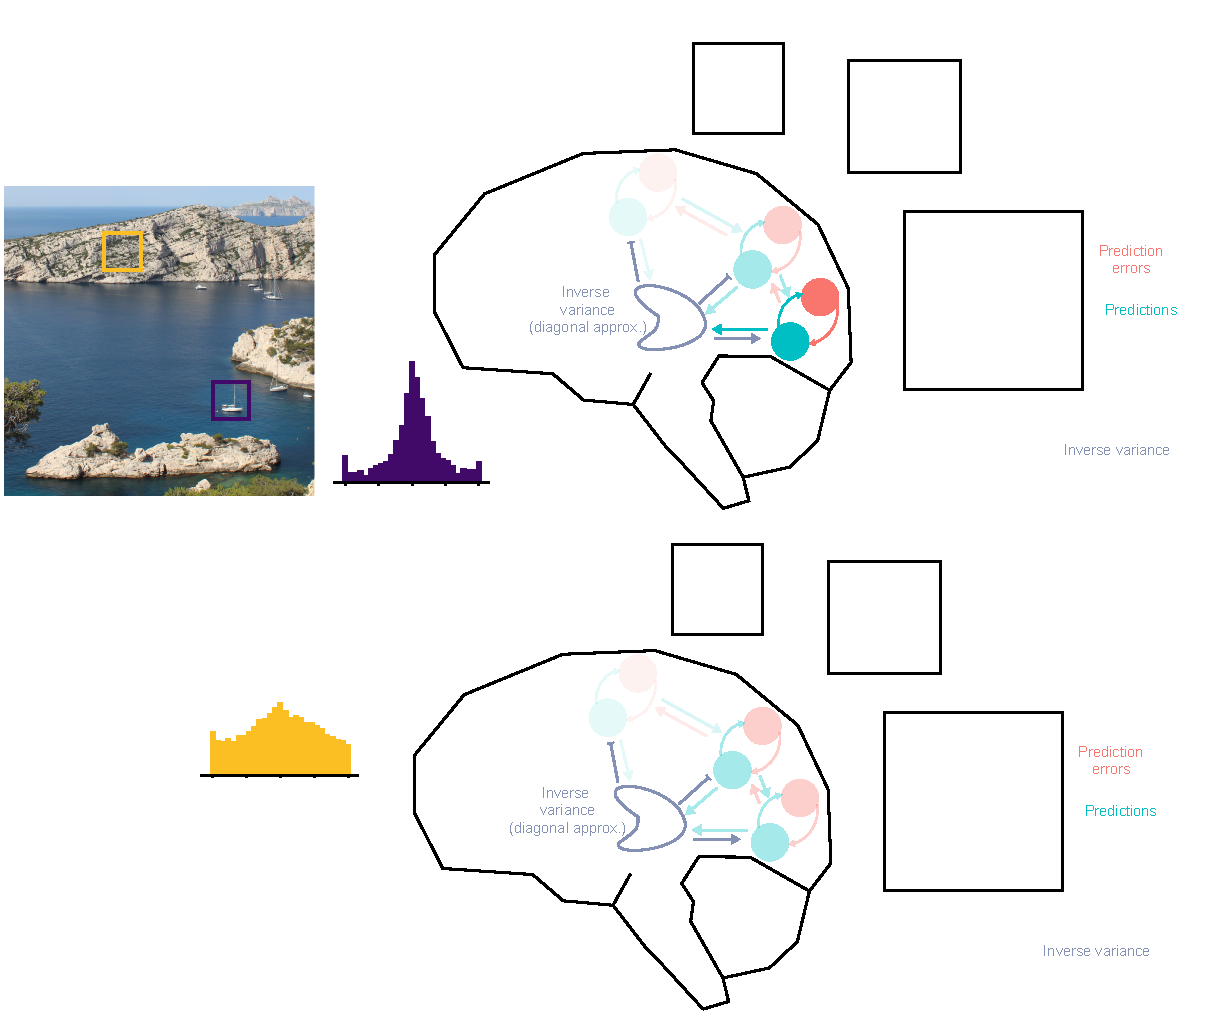
\includegraphics[width=1.\textwidth]{fig/fig_chap8_megamodel.pdf}
%\caption[Active modulation of neurons by orientation variance.]{Modulation of tuning curves by orientation variance. TODO.}
%\label{fig_chap8_megamodel}
%\end{figure} % figure that encompasses everything

This conceptual model also speaks to a number of testable hypotheses that can pave the way for exciting future research perspectives. But first, let us review the possible interpretations of this work, under both at the neurobiological and the computational front.



\section{Interpretation}
Although neuroscience has been historically based on studies related to how neurons encode only scalar approximate representations of their environment~\cite{sherrington1906observations, hubel1959receptive, o1971hippocampus}, theoretical~\cite{barlow1961possible} and experimental~\cite{leon2012motion} convergences have made it possible to start considering the full statistical nature of the environment we live in. The current research on inverse variance-weighting in the brain has exciting fundamental and clinical perspectives, which relates to two major avenues of interpretations. 



\subsection{Neurobiological Relevance}
At its core, inverse variance-weighting addresses the essential balance between internal priors and external perceptions. In the context of predictive processing, this mechanism guides the brain in discerning which of its predictions are reliable, and which it should discard in favor of prediction errors which warrant new attention. Interestingly, this dynamic can be seen as a foundational descriptor for several psychiatric disorders~\cite{friston2023computational}, including autism and schizophrenia.

\begin{figure}[h!tbp]
\vspace{0.1cm}
\centering
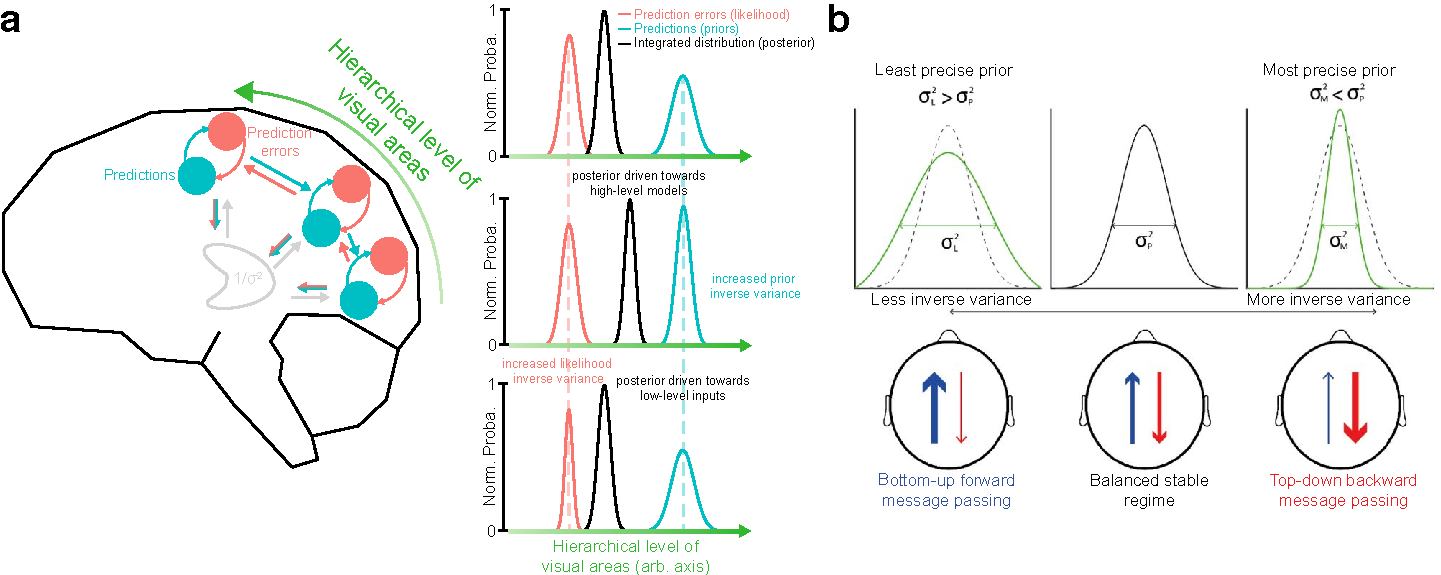
\includegraphics[width=1.\textwidth]{fig/fig_chap8_autism_schizo.pdf}
\caption[Message passing and computational psychiatry.]{Computational psychiatry under predictive processing.
(a) Message passing in the hierarchical Bayesian visual cortex. Under abnormally high inverse variance of the prior (second row), posterior is driven towards the internal models. Oppositely, high inverse variance of prediction errors (third row), drives posterior towards the sensory input. These respectively account for positive symptoms in schizophrenia and autism. 
(b) Same as (a), but in terms of bottom-up and top-down message passing, reproduced from~\cite{alamia2023oscillatory}.}
\label{fig_chap8_autism_schizo}
\end{figure} % figure for the inverse variance modulation + almia figure 1 from schizo paper

First, on a clinical level, recall that in the introduction (Figure~\ref{fig_chap2_equi_proba_var}), we discussed the notion that the variance of either prediction or prediction errors could drive the posterior likelihood towards one or the other. Under that generic description, hypersensitivity to external inputs, as is present in autistic spectrum disorders, can be conceptualized as a condition that drives overly precise prediction errors, overriding any possible internal models of the world. Typically, overlooking prediction error with no consequence for our inner model is something that we all do on a daily basis. In complex but non-threatening scenarios like social interactions, some errors are acceptable for broader understanding, and are part of the human social basis for learning. Inflexible processing of prediction errors in autism, due to impossibility of lowering their inverse variance-weighting in the decision process, leads to inability in ensuring "predictive success in an unpredictable world"~\cite{van2014precise}.

On the other end of the possible symptoms captured by inverse variance models lies schizophrenia. Hallucinatory experiences and feeling of disconnection with the external world~\cite{insel2010rethinking} are the hallmark of high weighting given to internal models over external likelihoods~\cite{sterzer2018predictive}. This is further supported by evidences that many of these symptoms align closely with the lesions of the neural substrate we described here, notably, visual perception and visual cognition being affected by pulvinar lesions~\cite{dorph2017postmortem}. Functional connectivity in schizophrenic patients have revealed reduced connectivity between the medial pulvinar and the frontal cortex~\cite{penner2018higher,yamamoto2018aberrant}. In the general model proposed earlier in this thesis, this would mean a compromised ability to regulate the flow of neuronal information between cortical areas by means of inverse variance weighting. Conversely, it could provide an evolutionary basis for the need for a central structure involved in the regulation of this mechanism, with a size proportional to that of the cortical areas being regulated~\cite{casanova2004functions}.

Second, on a cognitive level, another contribution of this thesis is to also offer a shift of our understanding of attention mechanisms, envisioning them as inverse variance mechanisms. Instead of conceptualizing recurrence and lateral inhibition as neural basis for sensory sharpening, one could consider that these are instead sampling mechanisms to drive (local) emphasis on the optimal percepts. 
Under this view, an interesting link is also to be made with the neuromodulatory activity, classically related to attention. Dopamine, for instance, is suggested to be crucial for the precision-adjustment of prediction errors, which in turn signals the significance of sensory inputs~\cite{fiorillo2008temporal, schultz1997neural}. Other neuromodulatory mechanism, such as cholinergic systems, can increase the gain of cortical neurons in response to sensory inputs~\cite{vaucher1997cholinergic, brown2011active}, and are thus tied to attentional mechanisms~\cite{kang2014boosting}. In that sense, these systems could be thought of as a third-order implementation of modulation by inverse variance, right after the first-order local recurrent interactions, second-order vision-centric pulvinar pathways, and serving to implement diffuse cortex-wise computations of inverse variance. 

Third, on a fundamental level, the dynamics of the activities that have been examined so far, as well as their propagation methods, their intracortical nature, all point towards an exciting research perspective for travelling waves. As introduced in chapter 4, traveling waves represent the dominant way of propagation of activity within the cortex. These waves facilitate processes like priming and suppression, but their exact role remains somewhat ambiguous and polymodal~\cite{muller2018cortical}. Similarly to the idea of a cholinergic mechanism, travelling waves also modulate the excitation/inhibition balance of the cortical activity rhythmically, which gates perceptual inference~\cite{dugue2011phase}. At the cortical area level, one contribution of this thesis is to consider that these waves might also implement a local inverse variance-weighting phenomenon, which offers a fresh perspective on their function in the cortex. At the macroscale, waves travelling between cortical areas, could also reveal mechanisms of propagation of inverse variance-weighted message, controlled by a series of locally weighted predictive oscillators~\cite{alamia2019alpha}. Specific changes in inverse variance could lower the excitability of prediction error units in the lower end of the hierarchy (i.e., in \gls{V1}), which would increase the preponderance of backward traveling waves, and correlates nicely with attentional experiments~\cite{alamia2019alpha}. One limitation here is that we have chosen to limit ourselves to an alpha/gamma duo, which is an oversimplification, and does not consider the fact that attentional visual search tasks correlates with even lower frequency rhythms, like theta~\cite{senoussi2019attention, michel2022distinct}. Given the tight relationship between unpredictable environment and the need for attentive search in feature space, this offers an interesting experimental perspective on manipulating visual variance, and correlating neural activity at the scale of the brain with the need to drive away - or close to - the input likelihood from posterior distributions. This will be discussed further in the final section of this manuscript.



\subsection{Machine Learning Relevance}
Inverse variance-weighting plays a significant role in both statistical and machine learning research~\cite{murphy2012machine}. Under this interpretation, inverse variance provides distinct advantages to a model, without implementational drawbacks (as studied in the neuroscientific context here). Indeed, given the mathematical triviality to compute a correlational matrix and inverse it, modelers obtain all the theoretical advantages described so far, with none of the complications related to recurrent neural message passing. One key advantage of implementing a degree of variance to a model's decision is to allow the readout of the model's confidence in its output. This can be as straightforward, in a deep neural network, as computing the sum of the variances in all layers, such that a network that has learned a precise representation of the environment returns a globally low variance of its activity.

Recently, the importance of associating confidence levels with algorithmic decisions has grown, placing inverse variance-weighting at the forefront of machine learning algorithm development. While there might be lighthearted examples, such as deep learning models mistakenly classifying an image of a panda with a single modified pixel as a dog, the stakes are much higher in practical industrial applications. As the research shifts towards implementing safety-critical neural networks, the emphasis on variance-weighted decisions becomes paramount. To quote Kendall and Yarin~\cite{kendall2017uncertainties}:  
\begin{flushleft}
    \textit{''Mappings are often taken blindly and assumed to be accurate, which is not always the case. In (\ldots) recent examples, this has had disastrous consequences. In May 2016 there was the first fatality from an assisted driving system, caused by the perception system confusing the white side of a trailer for bright sky. If (\ldots) these algorithms were able to assign a high level of uncertainty to their erroneous predictions, then the system may have been able to make better decisions and likely avoid disaster.''}\\
    from \fullcite{kendall2017uncertainties}
\end{flushleft}

Incorporating explicit learning rules based on variance into data modeling undeniably introduces additional complexity. As we have shown in the introduction of this manuscript and in the conclusion of chapter 5, these merely require simple additional considerations, and are compatible with current neural network frameworks. In that note, leading Deep Learning frameworks have already integrated support for Bayesian learning~\cite{paszke2017automatic}, which are soon bound to overtake regular Deep Learning in popularity~\cite{baldwin2022deep}.

A promising pathway to bridge explicit variance learning rules and neurobiology lies in predictive coding models. These models empirically approximate gradient backpropagation, a cornerstone technique for training deep neural networks (see chapter 3), across arbitrary computational graphs~\cite{millidge2022predictive}. This suggests that practically any deep neural network could be trained using units dedicated to predictions and their errors. Practical applications of this theory are already evident in simpler datasets like MNIST~\cite{millidge2020relaxing}. Notably, as we detailed in the conclusion of chapter 5, the implementation of inverse variance-weighting in this context is a novel proposition, as identity matrices are often use for simplicity's sake. The programming of these networks is elegantly simple - less than 100 Python code lines for an implementation as mathematically framed here~\cite{millidge2020relaxing}. On modern hardware, they also achieve comparable accuracy and convergence speeds to traditional backpropagation techniques.

Moreover, predictive coding's use in causal inference (as a generative model) could shed new light on how neural networks simulate and analyze dynamics within their nodes. In the recent context of Large Language Models, the inherent flexibility of predictive coding models allows any unit in the network to be set as a latent variable, endowing these models with the ability for flexible internal conditioning. This would enhance steerability over the network, for desirable safety purposes. The generative nature of these models also equips them to deal with incomplete inputs or outputs, a situation which typically requires expensive data curation by humans in the context of Deep Neural Networks. This attribute could be advantageous in creating models that infer missing information seamlessly. Finally, predictive coding also extends in a rather straightforward manner to arbitrary time-space variables, which allows for dynamical modelling, something which backpropagations techniques have always struggled with~\cite{millidge2022predictive}.

In the realm of hardware, the benefits of employing variance weighting through lateral inhibition might mirror those observed in neurobiology. Specifically, this method can offer computational allocation for significant, unpredictable fluctuations in data, while concurrently diminishing or sidestepping routine, predictable data streams. Highlighting these pronounced shifts could streamline the data transmitted across physical conduits, addressing a primary source of heat and computational inefficiency in neuromorphic chips~\cite{eshraghian2022memristor, rahimi2020complementary}. This could lead to faster, more energy-efficient neuromorphic networks that are particularly useful for edge computing, which, arguably, might also be why they are also implemented in the first place in the brain. Such asymmetrical message-passing structure is also reflected in the activity of \gls{V1}, notably, in the rasterplots presented in chapter 4.



\section{Limitations of the Studies}
The elaboration of a doctoral manuscript requires the doctoral candidate to perform scientific work, but also to learn how to even do such scientific work in the first place. As such, the erudite reader might have already spotted a number of suboptimal procedures in the experiments which are intrinsically bound to the learning curve the author went through. On a positive note, none of these limitations are unsurmountable roadblocks, and most of them can serve to formulate useful hypothesis for future research directions.

First and foremost, there is an intrinsic limit in the interpretations one can give from the experiments carried in chapter 4. Such extracellular recordings were performed under anesthesia, which yields heavy modulations of the activity of neurons~\cite{villeneuve2003use}. We have addressed this limitation in the conclusion of chapter 4's article, citing examples of experiments that were successfully translated from anesthetized to awake animals. One key neurophysiological element is however missing. Convincing experimental proofs have been published during the thesis, showing that the main effect of anesthesia is to decouple basal and apical dendrites of layer V cortical neurons~\cite{suzuki2020general}. Further, since pharmacological agents modulating the internal representations of the brain (i.e., predictions) have been shown to target specifically these same neurons~\cite{heindorf2022reduction}, it seems evident that one part of the prediction/prediction error network was heavily modulated in our experiments. Carrying experiments in awake, vigil animals is one way to address this limit, and the experiments in chapter 5 are a fair proof that chapter 4's study can yield interesting insights into a more ecologically relevant setting.

However, these experiments were carried with Utah Arrays (see chapter 4 and 5), which means a complete loss of information of the laminar position of neurons recorded. As such, we currently have no proof of a laminar-dependent inverse variance computations in awake cortex of primates. Change of coupling in deep layers might make for a very compelling case, which could be that inverse variance is also computed for predictions in layer V. Anatomically, there is actually as much, if not more (proportionally) recurrent connectivity between neurons of layer 5 of different neighboring cortical columns~\cite{briggs2011corticogeniculate, bastos2012canonical}. Functionally, layer V recurrent interactions also support very complex types of computations\cite{velez2014stimulus}, which are unique to these layers (some similarities exist~\cite{galloni2020apical}). This fully-lateral model of the cortex will be the central point of future research direction, and will be discussed in the next Perspectives section. 

Second, the choice of recording local, laminar, extracellular potentials is clearly not ideal for studying recurrent interactions. Using a better suited method would have required to know beforehand that recurrent interactions can carry out inverse variance weighting in the cortex, which was only hinted at by speculative models~\cite{bastos2012canonical, friston2005theory}. As such, a vast portion of neuronal "dark matter" was not observed, but only inferred. In a sense, this serves the interdisciplinar argument of this manuscript, which uses computational models to overcome experimental limitations. Now that these recurrent principles have been fairly well established, optical methods would be much better suited to study the inverse variance weighting mechanism in the cortex. One could expect some very interesting parallels between the results presented here, and the travelling waves (see chapter 4) observed both at the cortical area scale~\cite{chavane2011lateral} and at the brain scale~\cite{muller2018cortical, alamia2019alpha}. In terms of dynamics, travelling waves propagate locally with speeds that are coherent with the idea of a series of iterative recurrence-based computations~\cite{chavane2011lateral, chavane2022revisiting}. This possesses interesting ties with predictive processing, because local recurrence can allow a visual map to predict future position of a moving object through local interactions~\cite{britten1992analysis}, which is actually embedded within a travelling wave~\cite{benigno2023waves}. This experimental limitation, and its possibles interpretations in terms of travelling waves, will form part of the research perspectives discussed in the next section. 

%Third, there exists a limit in the assumptions used in the mapping of neurobiological elements for predictive processing. Since the inception of this thesis, there has been convincing biological experiments showing that prediction errors units are not only present in supragranular layers~\cite{keller2018predictive}, but also in deeper layers~\cite{heindorf2022reduction}. This could call for a major revision of the classical Bastos microcircuit model~\cite{bastos2012canonical}, which segregated the prediction and prediction errors to distinct layers, towards a model with duplicated compartments that essentially give the network a "teaching" signal for each cortical area, duplicated across layers % this makes no fucking sense but then again i've commented it out. the idea is that you duplicate the PE/P circuit twice so that you double the layer, and L2/3 serves to run a putative model of the environment that drive a predictive model int he deeper layers



\section{Perspectives for Future Research}
To conclude this thesis, we will develop here two major research perspectives that have stemmed from the present findings, and that are actively under study at the time of this writing. The first perspective stems from chapter 4 and 5 experiments, and concern extension of this thesis' work to rodent models. The second perspective is more ambitious, and better suited for exploration during a post-doctoral tenure. Both trajectories engage with the notion that existing models of recurrent connections in the cortex may be either limited by primate-centric considerations, or could simply be fundamentally unable to account for the meso-scale implementation of message passing in the cortex.

\subsection{Precision-Weighting without an Orientation Map}
The take-home message of this manuscript is that recurrence between specifically clustered groups of cells in orientation space mediates the computation of the inverse variance of orientation in \gls{V1}. But, how can these computations take place when there is no such thing as a specifically clustered groups of cells ? This is a non-trivial question, as this seemingly random architecture constitutes the organization of rodents' salt-and-pepper \gls{V1}. While primates and felines have clustered orientation processors organized in a map, which emerges through their heavy reliance on vision, rodents instead rely on whisker sensing, and thus lack a topologically structured orientation selective activity. Their somatosensory cortex, which processes information from the whiskers, do follow a topological structure. The extension of inverse variance-weighting in rodent cortex could be achieved by designing a class of stimulus similar to Motion Clouds, in the texture domain, and observe whether the variance-weighting in \gls{V1} holds in the somatosensory domain.

Back to the visual cortex, preliminary results from the co-authors Lamyae Ikan and Nelson Cortes suggest that mice do not exhibit any type of resilience to increased sensory variance, contrary to felines (chapter 4) and primates (chapter 5). If we put this under the notion that structured cortical recurrence is needed for such computations, this is one more argument in favor of this thesis' hypothesis. If we put this in the general predictive coding notion that high variance input are "explained away" and do not update the model, then it would be interesting to see what happens behaviorally. Even without processing of variance, does Bayesian inference still occur, and does the animal discard entirely its sense of vision to rely on its whiskers ? 

This also speak to an interesting property of resilience to general sources of uncertainty, as opposed to solely variance. Rodents do not possess orientation maps, but do possess individual neurons strongly tuned to specific orientations, with functional properties such as contrast invariance like primates~\cite{finn2007emergence}. This shows that an orientation map is not crucial for feature sensitivity, nor for maintaining contrast invariance. Changes in contrast, much like changes in orientation variance, are a source of visual uncertainty. Both type of uncertainty seem to affect \gls{V1} in the same way, at least in the pionnering study of Goris et al.~\cite{goris2015origin} (see also Figure~\ref{fig_chap8_mouse_mc}.
There is then a discrepancy between the notion that activity in primate \gls{V1} is similarly influenced by uncertainty of orientation (variance) and luminance (contrast), and the fact that mice are resilient to the latter but not the former. Contrast invariance mechanisms are a very popular topic in visual neuroscience, and there exists many theories on the emergence of contrast-invariant activity in \gls{V1}~\cite{vidyasagar2015origins}. While some authors suppose that cortical interactions could create contrast invariance~\cite{troyer1998contrast}, others have supposed that non-linearity in the thalamo-cortical connections from the \gls{LGN} is responsible for contrast invariance~\cite{finn2007emergence}. It would seem that, given this uncoupling between variance and luminance, the latter hypothesis would be better supported by our results.

\begin{figure}[h!tbp]
\vspace{0.1cm}
\centering
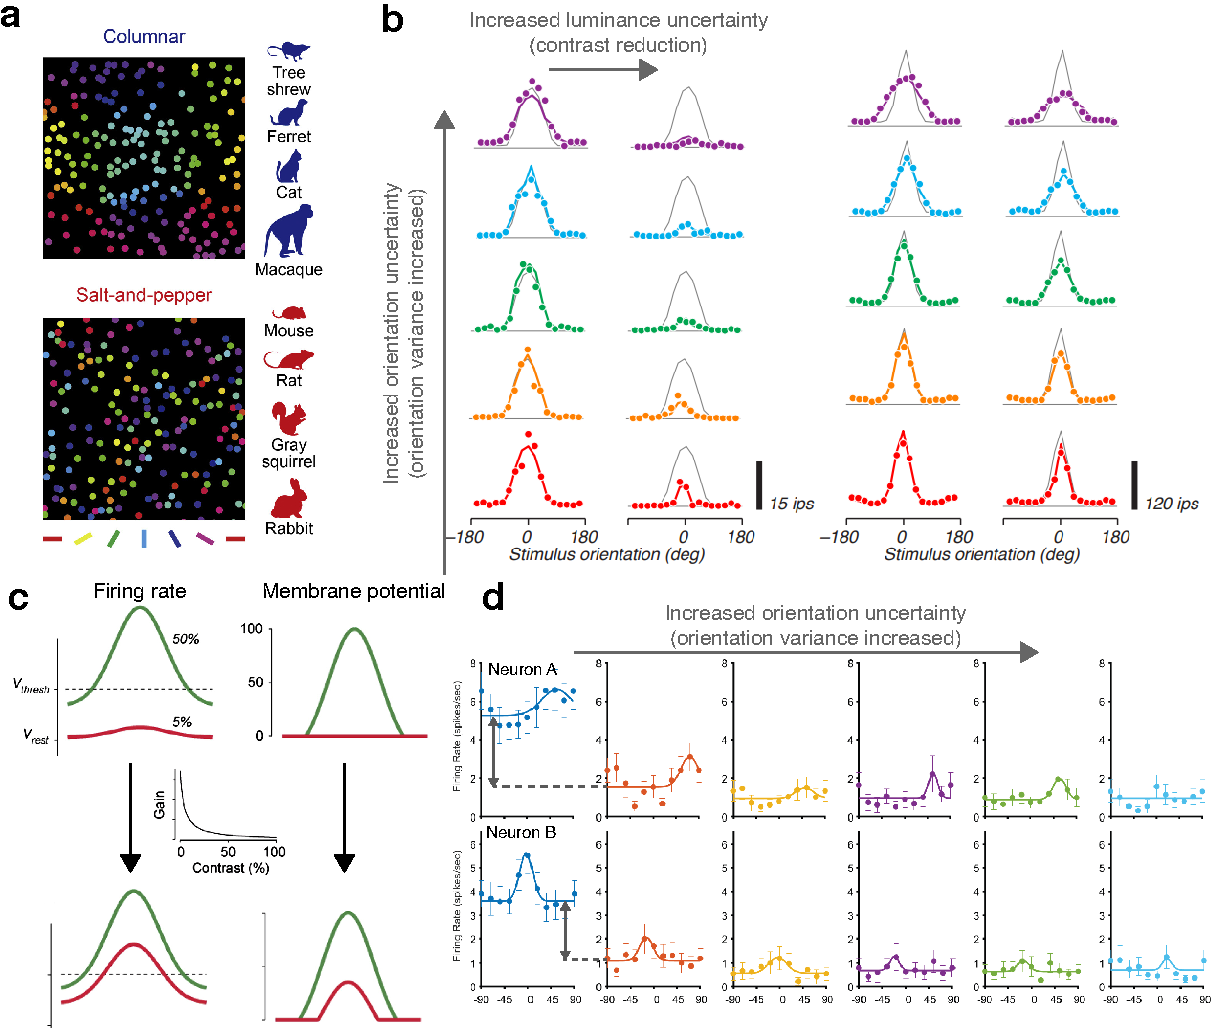
\includegraphics[width=1.\textwidth]{fig/fig_chap8_mouse_mc.pdf}
\caption[Contrast and orientation invariance in mouse\gls{V1}.]{Contrast and orientation invariance in mouse \gls{V1}. (a) Salt-and-pepper organisation of \gls{V1}, from~\cite{jang2020retino}. (b) Similar effect of contrast and orientation invariance on two primate \gls{V1} neurons, from~\cite{goris2015origin}. (c) An example of non-linear gain model that accounts for contrast resilience in \gls{V1}, from~\cite{finn2007emergence}. (d) Example of mice \gls{V1} neurons, showing a massive decrease in firing rate (arrows) with increased orientation variance (courtesy of Nelson Cortes). }
\label{fig_chap8_mouse_mc}
\end{figure} % figure about salt and pepper maps, contrast invariance


\subsection{The Microcircuit is Dead, Long Live the Microcircuit}
The theoretical framework upon which we have built our hypotheses, predictive processing~\cite{rao1999predictive,friston2005theory}, offers a solid mathematical basis to understand cortical functions. The accurate mapping of theory to biology, however, remains speculative~\cite{bastos2012canonical,shipp2016neural}, aside from accurate understanding of the prediction error circuits~\cite{keller2012sensorimotor, keller2018predictive}. Recall that earlier in the text, we mentioned recent findings by Heindorf and Keller~\cite{heindorf2022reduction}, who, utilizing antipsychotics and widefield calcium imaging in behaving mice, have demonstrated that antipsychotic drugs selectively impact Layer 5 neurons. As antipsychotics should target the neural elements responsible for internal representations~\cite{friston2018does} (i.e., predictions), this argues in favor of Layer 5 as the seat of predictions in the cortex. This is in line with the speculative layout of predictive coding in the cortical microcircuit~\cite{bastos2012canonical} (Figure~\ref{fig_chap2_microcircuit}). Yet, the effect of antipsychotics is selective to Layer 5, and leaves superficial layers unaffected. This poses a significant challenge to the established model of a series of hierarchically organized vertical microcircuits, derived from the columnar model of the cortex (Figure~\ref{fig_chap8_lateral}).

Namely, the canonical microcircuit~\cite{martin1994brief} posits an input in Layer 4, followed by a processing in Layer 2/3, which is then sent to a higher order cortical area's Layer 4. This challenge is not recent, as the vertical microcircuit as always had scientific opposition~\cite{horton2005cortical}, mostly on functional basis. Support for a new "horizontal microcircuit" perspective is now further bolstered by anatomical studies, which revealed a bidirectional flow of pathways segregated into two supra- and infragranular streams~\cite{markov2014anatomy}. This makes intuitive evolutionary sense, given that the appearance of six cortical layers is thought to result from a duplication of a three-layered structure~\cite{shepherd2011microcircuit}. It thus becomes increasingly plausible that neural activity is focused on integrating disparate features to construct probabilistic representations of the environment, rather than integrating information within a vertical microcircuit. This is evidenced not only by the fact that horizontal communication is the dominant mode of the cortex~\cite{muller2018cortical}, but also by the fact that inverse variance weighting requires a horizontal (recurrent) communication system~\cite{ladret2023cortical}.

\begin{figure}[h!tbp]
\vspace{0.1cm}
\centering
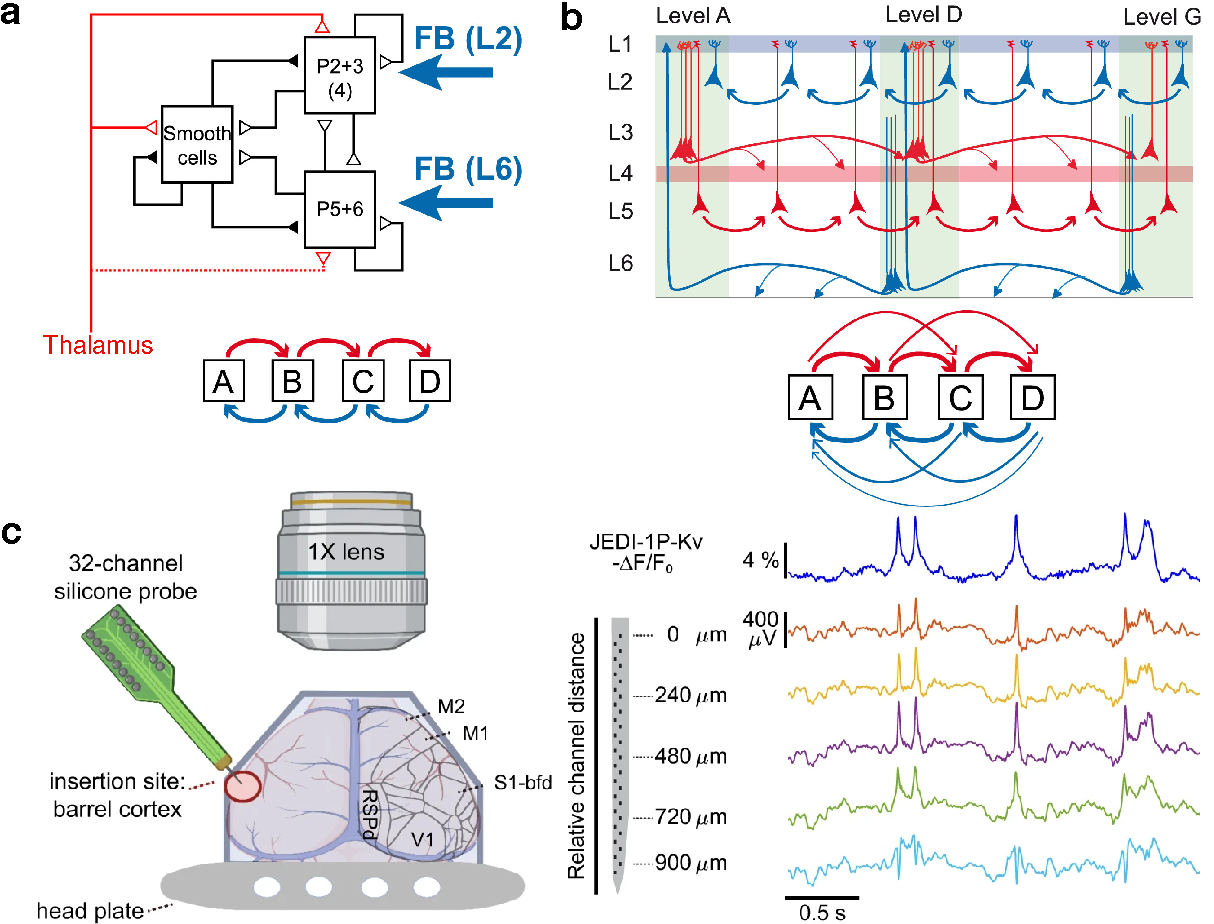
\includegraphics[width=1.\textwidth]{fig/fig_chap8_lateral.pdf}
\caption[Towards a horizontal microcircuit.]{Towards a horizontal microcircuit. (a) Canonical microcircuit of \gls{V1}~\cite{martin1994brief} (top) and assumed but wrong serial communication between area (bottom). (b) The cortex instead projects in two counterstreams that densely connect every area to one another. Adapted from~\cite{markov2014anatomy}. (c) Recording from a Genetically Encoded Voltage Indicators correlate with silicon probes, as used in this thesis, allowing for KHz-fast widefield imaging of the communication throughout the cortex, from ~\cite{lu2023widefield}.}
\label{fig_chap8_lateral}
\end{figure} % figure about salt and pepper maps, contrast invariance

In light of these evidences, it is essential to address the implications they hold for the cortical model of the canonical microcircuit, particularly as they propose both an extension and a challenge to the results of this thesis. If Layer 5 neurons have been affected due to anesthetic decoupling, as proposed above ~\cite{suzuki2020general}, the impact of this experimental limitation is more significant than previously thought. These neurons might not have just been part of a vertical microcircuit, but could have been an integral component of an independent horizontal deep circuit altogether, with an independent recurrent dynamic. Additionally, the manipulation of the variance of Motion Clouds and sensory inputs might have focused the present work on the inverse variance-weighting of prediction errors, rather than a combined investigation that includes both prediction errors and sensory inputs. This focus could have led to the inability to read out input variance from deep cortical layers in chapter 4. If we wish to amend this, there is an intrinsic technological challenge for current research methods of investigation (Figure~\ref{fig_chap4_chemla}).

Sampling the recurrent activity of inverse variance-weighting throughout the cortex, not at the scale of a single area, but at the dominant scale of cortex-wide activity, requires an experimental paradigm shift. This involves sampling widefield activity at the Nyquist frequency of the fastest signals required, i.e., $\approx 50$Hz gamma-band prediction errors (Figure~\ref{fig_chap7_oscillations}).
The advent of advanced optical methods now permits kHz-level recording of brain activity using Genetically Encoded Voltage Indicators. Wide-field microscopy techniques enable the observation of awake, behaving mice, granting comprehensive access to the visual cortex's surface. By employing genetically specific constructs, it is possible to isolate recordings to deep or superficial cortical layers~\cite{lu2023widefield}. Through such recordings of traveling waves, we can apply the vast body of literature on brain oscillations to living neural activity. 

This approach aligns with the theoretical models illustrated in Figure~\ref{fig_chap7_oscillations}, facilitating manipulation of the sensorium of behaving brains to pinpoint the anatomical seat of internal neuronal representations. Correlated with the known existence of prediction error circuits, this is the next scientific step for predictive coding, which has already achieved Marr's algorithmic~\cite{friston2005theory} and computational~\cite{sprevak2021predictive} levels, and is now poised to achieve implementational level, through a wholistic mapping of the neural elements of predictive coding.